\documentclass{article}
\usepackage[utf8]{inputenc}
\usepackage{amsmath,amsthm}
\usepackage[inline,shortlabels]{enumitem}
\usepackage{fancyvrb}
\usepackage{graphicx}
\usepackage{hyperref}
\usepackage{subcaption}
\usepackage{tikz}

\newtheorem{thm}{Theorem}[section]
\theoremstyle{definition}
\newtheorem{Def}{Definition}[section]
\theoremstyle{remark}
\newtheorem{Rmk}{Remark}[section]
\newtheorem*{Nt}{Note}

\title{Latex Certificate Course Instructions}
\author{Jacob Antony}
\date{\today}

\begin{document}

\maketitle

\section{Cross Reference}
	\LaTeX{} has a mechanism to refer different elements of the same document. You can refer to equations, sections, tables and figures. The \texttt{\textbackslash label} command is used to create an anchor of reference. And \texttt{\textbackslash ref} command is used to refer to such an anchor. Also \texttt{\textbackslash pageref} command is used to refer to the page number of that anchor.
	
	You can have forward references as \LaTeX{} creates/updates anchors in the associated \texttt{aux} file. And updates the references using the existing labels in the \texttt{aux} file. You might have to compile twice to update labels which are newly introduced.

\subsection{Associated Files}
	There are many associated files created and managed by \LaTeX{} for generating your document. The files with \texttt{tex} extension are \LaTeX{} source files where you write your \LaTeX{} file for document creation. The \texttt{pdf} extension is used to the PDF files generated by \LaTeX{}. 

	We can tell the purpose of each associated file from its file extension. The following are a few important file extensions,
\begin{description}
	\item[aux] Auxiliary Data for toc, reference, index, bibliography, \dots
	\item[log] Compilation Log --- Errors and Warnings
	\item[toc] Table of Contents
	\item[lof] List of Figures
	\item[lot] List of Tables
\end{description}

An ellaborate list of file extensions for different purposes, is available at \href{https://tex.stackexchange.com/questions/7770/file-extensions-related-to-latex-etc}{Tex StackExchange}.

\section{figure Environment}
	The \texttt{figure} environment is used for adding figures to your document. The \texttt{figure} elements can have captions. And you can place anchor on figure element for referencing.

\subsection{includegraphics Command}
	The \texttt{figure} environments are supposed to contain images that you draw using \LaTeX{} or that you already have in your computer.
	
	You can add images on your computer to the document using \texttt{\textbackslash includegraphics} command. This command takes the image address as argument and image dimensions and effects as optional arguments.

\begin{figure}[h]
\centering
\begin{subfigure}{0.45\textwidth}
\begin{Verbatim}[numbers = left]
\usepackage{graphicx}
...
\begin{document}
...
\begin{figure}
\centering

\includegraphics{flower.jpg}
\caption{Flower}
\end{figure}
\end{Verbatim}
\end{subfigure}
%\begin{subfigure}{0.45\textwidth}
\begin{subfigure}{0.45\textwidth}
\centering

\includegraphics[scale=0.05]{flower.jpg}
\caption{Flower}
\end{subfigure}
%\end{subfigure}
\caption{figure Environment}
\label{fig:figure}
\end{figure}

\subsection{Drawing using Tikz}

\begin{figure}[h]
\centering
\begin{subfigure}{0.45\textwidth}
\begin{Verbatim}[numbers = left]
\usepackage{tikz}
...
\begin{document}
...
\begin{figure}
\centering
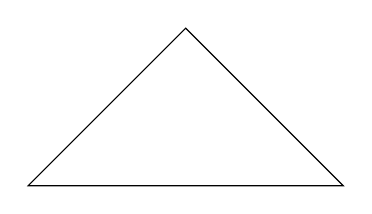
\begin{tikzpicture}
\draw (0,0) -- (2,2) %
-- (4,0) -- cycle;
\end{tikzpicture}
\caption{Triangle}
\end{figure}
\end{Verbatim}
\end{subfigure}
\begin{subfigure}{0.45\textwidth}
\centering
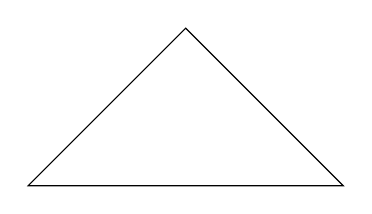
\begin{tikzpicture}
\draw (0,0)--(2,2)%
--(4,0)--cycle;
\end{tikzpicture}
\caption{Triangle}
\end{subfigure} 
\caption{Drawing using Tikz}
\label{fig:tikz}
\end{figure}


\end{document}

\begin{figure}[h]
\centering
\begin{subfigure}{0.45\textwidth}
\begin{Verbatim}[numbers = left]
...
\end{Verbatim}
\end{subfigure}
\begin{subfigure}{0.45\textwidth}
...
\end{subfigure} 
\caption{cap}
\label{fig:cap}
\end{figure}

\subsection{Cross-referencing}
Suppose you want to refer to an image/table in the same document on a different page. \LaTeX{} does have provisions for references. You are not yet there. You should mention page number explicitly as the page numbers might change as your add/remove sentences. 

Missing Contents
================
phantom, hspace, vspace,hrulefill, dotfill, rule, 
~ no line break \- possible line break

tikz - intentionally ignored
